\documentclass[11pt,ngerman,a4paper]{article}
%Gummi|061|=)
\usepackage{amsmath}
\usepackage{a4wide}
\usepackage{url}
\usepackage{amsthm}
\usepackage{amsbsy}
\usepackage{amssymb}
\usepackage{inputenc}
\usepackage{rotating} 
\usepackage{graphicx}
\usepackage{paralist}
\usepackage{selinput}
\SelectInputMappings{%
adieresis={ä},
germandbls={ß},
}
\title{\textbf{Versuch V351: Fourier-Analyse und Synthese}}
\author{Martin Bieker\\
		Julian Surmann\\
		\\
		Durchgef\"{u}hrt am 16.01.2014\\
		TU Dortmund}
\date{}
\usepackage{graphicx}
\begin{document}
\renewcommand\tablename{Tabelle}
\renewcommand\figurename{Abbildung}
\maketitle
\thispagestyle{empty}
\newpage
\clearpage
\setcounter{page}{1}


\section{Einleitung}
In der Physik werden manchmal periodische Signale gemessen, zum Beispiel Töne eines Musikinstruments. Mit Hilfe der Fourier-Analyse lässt sich dann ein Frequenzspektrum erstellen. An diesem kann man am Beispiel des Musikinstrumentes die Grund- und Obertöne sowie deren Amplituden bestimmen.
In diesem Versuch sollen zunächst periodische Signale mit dem digitalen Oszilloskop untersucht werden und anschließend eigene Signale erzeugt werden, die aus vorher berechneten Grund- und Oberschwingungen bestehen.
\section{Theorie}
\subsection{Fourier-Analyse}
Eine gleichmäßig konvergierende Reihe
\begin{equation}
\frac{a_0}{2}+\sum_{n=1}^\infty \left(a_ncos\left(\frac{2\pi nt}{T}\right)+b_nsin\left(\frac{2\pi nt}{T}\right)\right)
\label{formel1}
\end{equation}
stellt eine periodische Funktion $f(t)$ dar. Die Periodendauer beträgt T. Die Faktoren $a_n$ und $b_n$ werden errechnet mit
\begin{equation}
a_n=\frac{2}{T}\int\limits_{0}^{T}f(t)cos\left(\frac{2\pi nt}{T}\right)dt , n = 1,2,3,...
\label{an}
\end{equation}
\begin{equation}
b_n=\frac{2}{T}\int\limits_{0}^{T}f(t)sin\left(\frac{2\pi nt}{T}\right)dt , n = 1,2,3,...
\label{bn}
\end{equation}
Die Grundfrequenz der untersuchten Funktion ist $v=\frac{1}{T}$, die Oberschwingungen haben als Frequenz in der Regel ganzzahlige Vielfache von $v$.
Manchmal ist es möglich, Vereinfachungen anzuwenden. So könnte die zu analysierende Funktion gerade oder ungerade sein. Dadurch ergeben sich folgende Zustände:
\begin{equation}
gerade: f(t)=f(-t) \Rightarrow b_n=0
\end{equation}
\begin{equation}
ungerade: f(-t)=-f(t) \Rightarrow a_n=0
\end{equation}
Manchmal ist es auch möglich, eine Funktion in gerade und ungerade Teile aufzuteilen. In Abbildung \ref{spektrumtheo} sind die Amplituden der Teilschwingungen gegen die Frequenzen aufgetragen.
\begin{figure}[htp]
\centering
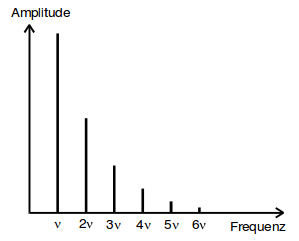
\includegraphics[scale=0.7]{abb/spektrumtheo.png}
\caption{Beispiel für ein Frequenzspektrum [1]}
\label{spektrumtheo}
\end{figure}
Bei periodischen Funktionen handelt es sich immer um ein Linienspektrum.
\subsection{Fourier-Transformation}
Die Fourier-Transformation ist in der Lage, ein vollständiges Frequenzspektrum einer Funktion zu errechnen. Diese Transformation funktioniert auch mit einer nicht periodischen Funktion. Das (kontinuierliche) Frequenzspektrum einer Funktion f(t) wird mit
\begin{equation}
g(\nu)=\int_{-\infty}^\infty f(t)e^{i\nu t}dt
\label{trafo}
\end{equation}
berechnet. Da hier aber theoretisch ein unendlich langes Signal benötigt wird (siehe Integration von $-\infty$ bis $\infty$), kommt es zu Abweichungen: $g(\nu)$ wird stetig und integrierbar, die "Linien" des Spektrums werden breiter.

\section{Vorbereitung und Durchf\"{u}hrung}
\subsection{Berechnung der Fouerierkoeffizienten}
Im Folgenden sollen die Fourierkomponenten von 3 verschiedenen Funktionen bestimmt werden. 
\paragraph{Dreicksfunktion}
Die Dreiecksfunktion ist definiert als
\begin{equation}
f \colon  \left[-\frac{T}{2}, \frac{T}{2}\right]\to \mathbb{R}, f(t) = 1 - \left|\frac{2t}{T}\right|.
\end{equation}
Abbildung \ref{org_hut} zeigt die periodische Fortsetzung dieser Funktion.
\begin{figure}[htp]
\centering
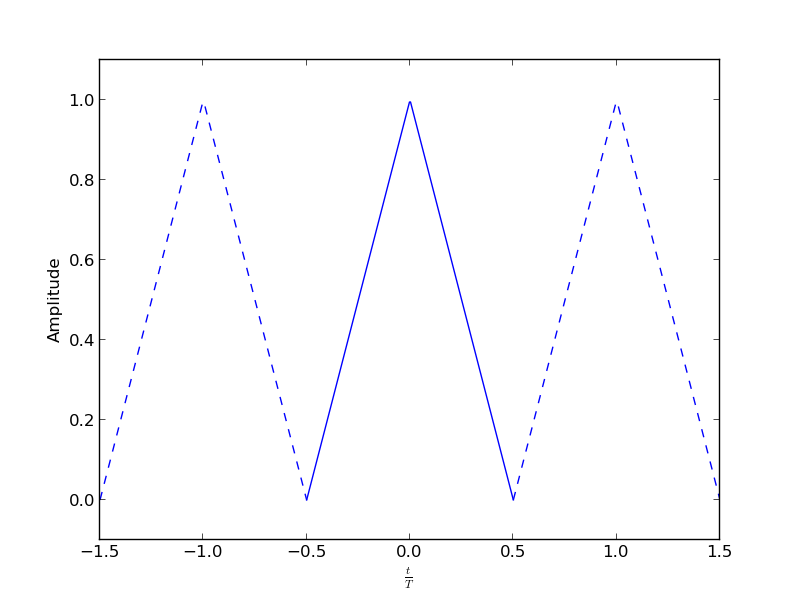
\includegraphics[scale=0.7]{abb/Abb2.png}
\caption{Periodische Fortsetzung der Dreicksfunktion}
\label{org_hut}
\end{figure} Da es sich bei dieser Abbildung um eine gerade Funktion handelt, sind alle Fourierkoeffizienten $b_n$ gleich null. Der Koeffizient $a_0$ betr\"agt nach Formel \ref{an}
\begin{equation} 
a_0 =\frac{2}{T} \int_{-\frac{T}{2}}^{\frac{T}2}\!f(t)\,\mathrm dt= \frac4T \int_{0}^{\frac{T}2}\!1-\frac{2t}{T}\,\mathrm dt= 1.
\end{equation}
F\"ur den Fall $n \neq 0$ folgt analog:
\begin{align}
a_n =\frac{2}{T} \int_{-\frac{T}{2}}^{\frac{T}2}\!f(t)cos\left(\frac{n2\pi t}{T}\right) \,\mathrm dt = \frac{4}{T} \int_0^\frac{T}2\!\left(1-\frac{2t}{T}\right)cos\left(\frac{n2\pi t}{T}\right)\,\mathrm dt \\= \frac{2 (1-(-1)^n)}{\pi^2n^2} = \begin{cases}
0 & n\mbox{ gerade} \\ \frac{4}{\pi^2n^2} & n\mbox{ ungerade}
\end{cases}
\end{align} 
\paragraph{S\"agezahnfunktion} Diese Abbildung ist durch
\begin{equation}
f \colon  \left[-\frac{T}{2}, \frac{T}{2}\right]\to \mathbb{R}, f(t) = t
\end{equation}
definiert. In Abbildung \ref{org_saw} ist die periodische Fortsetzung dieser Funktion zu sehen.
\begin{figure}[htp]
\centering
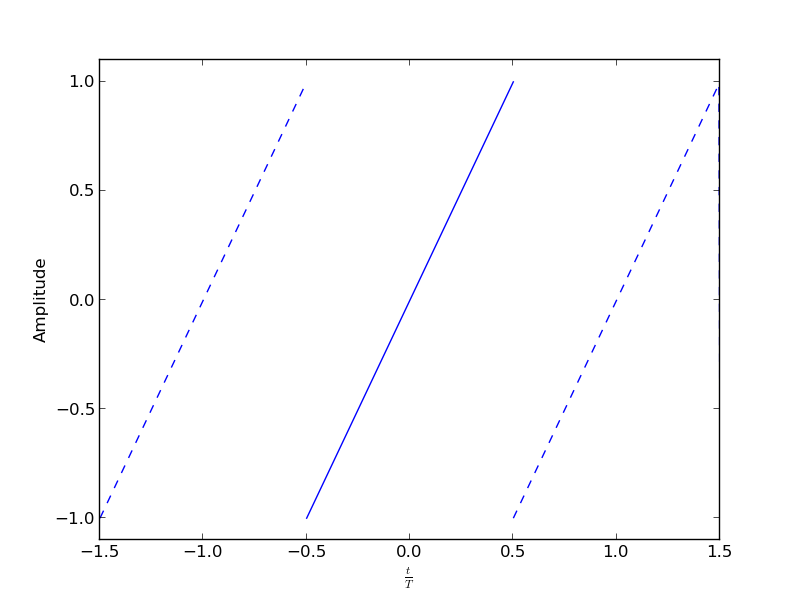
\includegraphics[scale=0.7]{abb/Abb1.png}
\caption{Periodische Fortsetzung der S\"agezahnfunktion}
\label{org_saw}
\end{figure} Da es sich bei dieser Funktion um eine ungerade Abbildung handelt, sind alle Koeffizienten $a_n$ gleich null. F\"ur die $b_n$ gilt nach Formel \ref{bn}:
\begin{align}
b_n = \frac 2 T\int_{-\frac T 2}^\frac T 2\!f(x)\,sin\left(\frac{n2\pi t}{T}\right)\,\mathrm dt = \frac 2 T \int_{-\frac T 2}^\frac T 2\!t\,sin\left(\frac{n2\pi t}{T}\right)\,\mathrm dt =\frac{ -2(-1)^n}{\pi n}\\=
\begin{cases}
-\frac{2}{\pi n} & n \mbox{ gerade}  \\
\frac{2}{\pi n} & n \mbox{ ungerade}
\end{cases}
\end{align}
\paragraph{Rechteckfunktion} Zur einfacheren Berechnung der Fourier-Koeffizienten wird diese Funktion als
\begin{equation}
f \colon  \left[-\frac{T}{2}, \frac{T}{2}\right]\to \mathbb{R},\,f(t) = \begin{cases}
-1 & \mbox{f\"ur } n < 0 \\
1  & \mbox{f\"ur } n \geq 0
\end{cases}
\end{equation}
definiert. Die Abbildung \ref{org_rect} zeigt die periodische Fortsetzung dieser Funktion. 
\begin{figure}[htp]
\centering
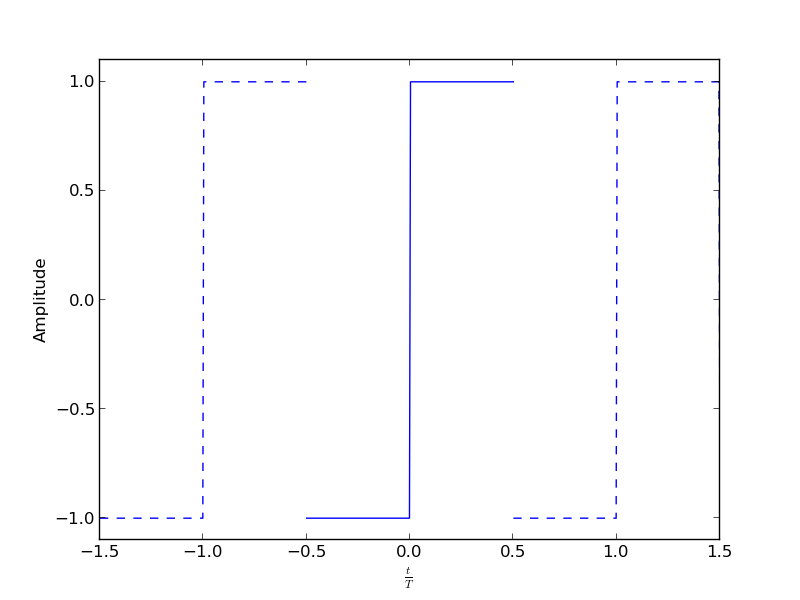
\includegraphics[scale=0.7]{abb/Abb3.png}
\caption{Periodische Fortsetzung der Rechteckfunktion}
\label{org_rect}
\end{figure}Da es sich auch bei dieser Funktion um eine ungerade Abbildung handelt sind analog zu oben alle $a_n$ gleich null. Des Weiteren sind die $b_n$ durch
\begin{align}
b_n = \frac 2 T\int_{-\frac T 2}^\frac T 2\!f(x)\,sin\left(\frac{n2\pi t}{T}\right)\,\mathrm dt = \frac 2 T \left[ \int_{-\frac T 2}^0\!sin\left(\frac{n2\pi t}{T}\right)\,\mathrm dt - \int_0^{\frac T 2}\!sin\left(\frac{n2\pi t}{T}\right)\,\mathrm dt \right] \\
= \frac{2 (1- (-1)^n)}{n \pi} =
\begin{cases}
0 & n \mbox{ gerade}\\
\frac4{n\pi} & n \mbox{ ungerade}
\end{cases} 
\end{align}
gegeben.
\subsection{Fourier-Analyse}

In diesem Versuchsteil sollen mit einem Funktionengenerator erstellte Funktionen mit dem digitalen Speicheroszilloskop untersucht werden. Dafür wird das Signal direkt in das Oszilloskop gespeist. Die "Math"-Funktion führt dann für ein einstellbares Zeitintervall eine Fouriertransformation durch. Dabei ist zu beachten, dass das Messintervall möglichst lang ist, um das Integral mit unendlichen Grenzen möglichst gut anzunähern. Die ersten neun von Null verschiedenen Maxima sollen dann abgelesen werden, um diese mit den theoretischen, im Voraus berechneten, zu vergleichen.

\subsection{Fourier-Synthese}

In diesem Versuchsteil sollen die verschiedenen Schwingungsformen aus ihren Fourierkomponenten zusammengesetzt werden. Dazu wird ein so genannter Oberwellengenerator verwendet. Dies ist ein Ger\"at, welches Sinusschwingungen mit festen Phasenbeziehungen und ganzzahligen Frequenzverh\"altnissen erzeugt. Zun\"achst werden dazu die Fourier-Keffizienten f\"ur die ersten 9 Oberwellen berechnet. Die Ergebnisse finden sich in Tabelle 1. Danach werden die richtigen Phasenbeziehungen zwischen den Oberwellen und der Grundschwingung hergestellt. Dazu wird je eine Oberwelle auf Kanal 1 und die Grundschwingung auf den zweiten Kanal eines Oszilloskops gegeben. Auf dieses Weise kann mit Hilfe von Lissajous-Figuren die richtige Phasenbeziehung zwischen den Schwingungen hergestellt werden. Die negativen Koeffizienten der S\"agezahnfunktion werden dabei durch eine Phasenverschiebung von $180 ^\circ$ realisiert. 

\noindent
Die Amplitudenverh\"altnisse der einzelnen Komponenten sollen so gew\"ahlt werden, dass die Grundschwingung jeweils die gr\"o\ss te Amplitude des Oberwellengenerators ($0.6\,$V) aufweist. Dazu werden die Fourier-Koeffizienten entsprechend skaliert. Alle Einstellungen am Generator, die zur Synthese der einzelnen Funktionen n\"otig sind, befinden sich zusammengefasst in Tabelle 2. Nachdem der Oberwellengenerator entsprechend eingestellt wurde, kann die Summenschwingung auf dem Oszilloskop betrachtet werden.
\section{Ergebnis}
\subsection{Fourier-Analyse}
Die vom Oszilloskop erstellte Analyse der Rechteckspannung ist als Beispiel in Abbildung \ref{recht} zu sehen.
\begin{figure}[htp]
\centering
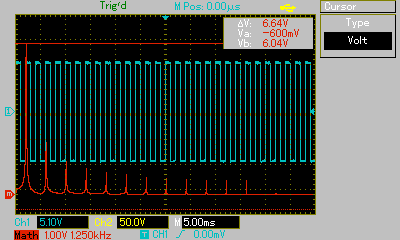
\includegraphics[scale=0.8]{Screenshots/MAP001.png}
\caption{Experimentelles Frequenzspektrum einer Rechteckspannung}
\label{recht}
\end{figure}
Die Tabellen \ref{hut} bis \ref{rect} zeigen die abgelesenen Amplituden sowie ein Vergleich zu den theoretisch berechneten Werten. Bei den Werten der Dreiecksfunktion sind die Amplituden sehr schnell sehr stark abgefallen, sodass ein genaues Ablesen der Werte deutlich erschwert wurde. Die rel. Abweichungen zeigen dies deutlich. Auch bei den anderen Funktionen liegt die Abweichung der experimentellen zu den theoretischen Werten bei bis zu 39\%.
\subsection{Fourier-Synthese} 
\paragraph{Grundschwingung} Die Grundschwingung f\"ur alle betrachteten Funktionen ist eine Sinuswelle mit einer Ampltude von $0.6\,$V. Diese ist in Abbildung 4 dargestellt.
\begin{figure}[h]
\centering
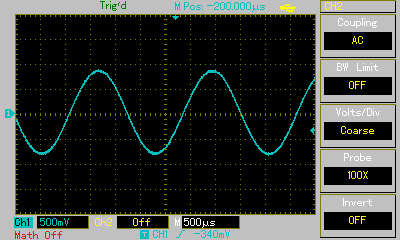
\includegraphics[scale=0.8]{Screenshots/basic.png}
\caption{Oszillogramm der Grundschwingung}

\end{figure}
\paragraph{Dreiecksfunktion} 
Abbildung \ref{hut_1} zeigt die Summenschwingung nach dem Einschalten der Oberwellen bis einschlie\ss lich $ n = 5$. 
\begin{figure}[htp]
\centering
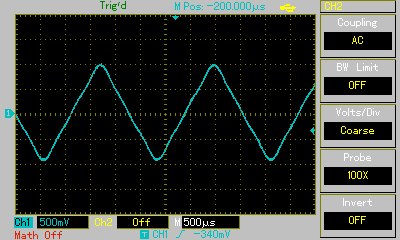
\includegraphics[scale=0.8]{Screenshots/hut_1.png}
\caption{Oszillogramm  der Summenschwingung bis $n = 5$}
\label{hut_1}
\end{figure}
Es ist erkennbar, dass sich die Summenschwingung sich sehr schnell der Dreiecksfunktion an\"ahert. Das Oszillogramm in Abbildung \ref{hut_2} zeigt die Summenschwingung, nachdem alle verf\"ugbaren Oberwellen eingeschaltet wurden.
\begin{figure}[htp]
\centering
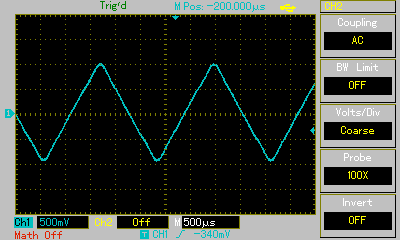
\includegraphics[scale=0.8]{Screenshots/hut_2.png}
\caption{Oszillogramm  der Summenschwingung bis $n = 9$}
\label{hut_2}
\end{figure}
 
\paragraph{S\"agezahnfunktion}
Abbildung \ref{saw_1} zeigt die Summenschwingung nach dem Einschalten der Oberwellen bis einschlie\ss lich $ n = 5$. 
\begin{figure}[htp]
\centering
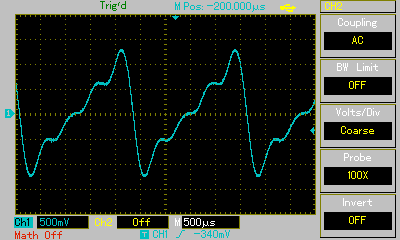
\includegraphics[scale=0.8]{Screenshots/saw_1.png}
\caption{Oszillogramm  der Summenschwingung bis $n = 9$}
\label{saw_1}
\end{figure}
Das Oszillogramm in Abbildung \ref{saw_2} zeigt die Summenschwingung, nachdem alle verf\"ugbaren Oberwellen eingeschaltet wurden. In dieser Grafik ist das Gibbsche Phänomen an der Sprungstellen deutlich zu erkennen.
\begin{figure}[htp]
\centering
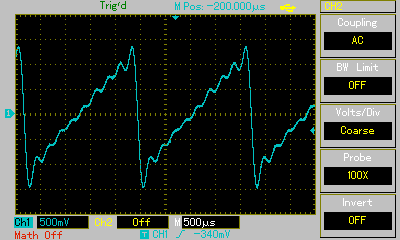
\includegraphics[scale=0.8]{Screenshots/saw_2.png}
\caption{Oszillogramm  der Summenschwingung bis $n = 5$}
\label{saw_2}
\end{figure}
\paragraph{Rechteckfunktion}
Abbildung \ref{rect_1} zeigt die Summenschwingung nach dem Einschalten der Oberwellen bis einschlie\ss lich $ n = 5$. 
\begin{figure}[htp]
\centering
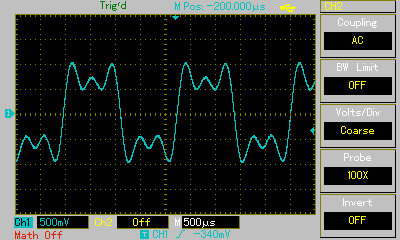
\includegraphics[scale=0.8]{Screenshots/rect_1.png}
\caption{Oszillogramm  der Summenschwingung bis $n = 5$}
\label{rect_1}
\end{figure}
Es ist erkennbar, dass sich die Summenschwingung der Zielfunktion an\"ahert. Das Oszillogramm in Abbildung \ref{rect_2} zeigt die Summenschwingung nachdem alle verf\"ugbaren Oberwellen eingeschaltet wurden. Auch bei dieser Funktion tritt ein \"Uberschwingen an den Unstetigkeitsstellen auf.
\begin{figure}[htp]
\centering
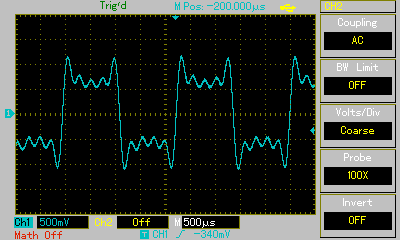
\includegraphics[scale=0.8]{Screenshots/rec_2.png}
\caption{Oszillogramm  der Summenschwingung bis $n = 5$}
\label{rect_2}
\end{figure}
\section{Diskussion}
Die Fourier-Analyse mit dem Oszilloskop hat gut funktioniert. Die Maxima waren gut ablesbar. Allerdings waren die Amplituden bei der Dreiecks-Funktion nur bis zum fünften Peak ablesbar, da die Amplituden zu stark abfielen. Die experimentell ermittelten Amplituden haben leider eine Abweichung von bis zu 39 \% zu den theoretischen Werten. Dies lässt sich nur teilweise mit der Messungenauigkeit erklären. Die Fourier-Synthese hat gut funktioniert.
\section{Abbildungsverzeichnis}
\begin{enumerate}[{[}1{]}]
\item Entnommen der Praktikumsanleitung "Fourier-Analyse und Synthese" der TU Dortmund. Download am 18.01.14 unter:\\
 \url{http://129.217.224.2/HOMEPAGE/PHYSIKER/BACHELOR/AP/SKRIPT/V351.pdf}
\end{enumerate}
\section{Anhang}
\begin{itemize}
\item Tabellen
\item Auszug aus dem Messheft
\end{itemize}

\newpage
\begin{table}
\centering
\begin{tabular}{|c|c|c|c|}

\hline
n & Dreieck [$a_n]$ & S\"agezahn [$b_n$] & Rechteck $[b_n]$ \\
\hline
1 & 0.405 & 0.637 & 1.273\\
2 & 0.0 & -0.318 & 0.0\\
3 & 0.045 & 0.212 & 0.424\\
4 & 0.0 & -0.159 & 0.0\\
5 & 0.016 & 0.127 & 0.255\\
6 & 0.0 & -0.106 & 0.0\\
7 & 0.008 & 0.091 & 0.182\\
8 & 0.0 & -0.08 & 0.0\\
9 & 0.005 & 0.071 & 0.141\\
\hline
\end{tabular}
\label{table1}
\caption{Fourier-Koeffizienten der verschiedenen Schwingungen}
\end{table}

\begin{table}
\centering
\begin{tabular}{|c||c|c||c|c||c|c|}
\hline
n & \multicolumn{2}{c||}{Dreiecksfunktion} & \multicolumn{2}{c||}{Sägezahnfunktion} & \multicolumn{2}{c|}{Rechteckfunktion} \\
 & Amplitude [V] & $\Delta \varphi\,[^\circ]$ & Amplitude [V] & $\Delta \varphi\,[^\circ]$ & Amplitude [V] & $\Delta \varphi\,[^\circ]$ \\
\hline
1 & 0.6 & 0 & 0.6 & 0 & 0.6 & 0\\
2 & 0 &  & 0.3 & 180 & 0& \\
3 & 0.067 & 0 & 0.2 & 0 & 0.2 & 0\\
4 & 0 &  & 0.15 & 180 & 0 & \\
5 & 0.024 & 0 & 0.12 & 0 & 0.12 & 0\\
6 & 0 &  & 0.1 & 180 & 0 & \\
7 & 0.012 & 0 & 0.086 & 0 & 0.086 & 0\\
8 & 0 &  & 0.075 & 180 & 0 & \\
9 & 0.007 & 0 & 0.067 & 0 & 0.067 & 0\\
\hline
\end{tabular}
\label{params}
\caption{Einstellungen des Oberwellengenerators für die jeweiligen Schwingungen}
\end{table}
\begin{table}
\centering
\begin{tabular}{|c|c|c|c|c|}
\hline
n & $a_n [V]$ & $(\frac{a_n}{a_1})_{exp}$ & $(\frac{a_n}{a_14})_{th}$ & rel. Abweichung\\
\hline
1&5.6 & 1.0 & 1.0 & 0.0\\
3&0.656 & 0.117 & 0.111 & 0.051\\
5&0.184 & 0.033 & 0.04 & -0.212\\
7&0.112 & 0.02 & 0.02 & 0.0\\
9&0.04 & 0.007 & 0.012 & -0.714\\
\hline
\end{tabular}
\label{hut}
\caption{Ergebnisse der Fourieranalyse für die Dreicksfunktion}
\end{table}

\begin{table}
\centering
\begin{tabular}{|c|c|c|c|c|}
\hline
n & $b_n [V]$ & $(\frac{b_n}{a_1})_{exp}$ & $(\frac{b_n}{a_1})_{th}$ & rel. Abweichung\\
\hline
1&2.94 & 1.0 & 1.0 & 0.0\\
2&2.34 & 0.796 & 0.5 & 0.372\\
3&1.02 & 0.347 & 0.333 & 0.04\\
4&1.16 & 0.395 & 0.25 & 0.367\\
5&0.07 & 0.022 & 0.2 & -8.091\\
6&0.80 & 0.272 & 0.167 & 0.386\\
7&0.52 & 0.177 & 0.143 & 0.192\\
8&0.60 & 0.204 & 0.125 & 0.387\\
9&0.46 & 0.155 & 0.111 & 0.284\\
\hline
\end{tabular}

\label{saw}
\caption{Ergebnisse der Fourieranalyse für die Sägezahnfunktion}
\end{table}

\begin{table}
\centering
\begin{tabular}{|c|c|c|c|c|}
\hline

n & $b_n [V]$ & $(\frac{b_n}{a_1})_{exp}$ & $(\frac{b_n}{a_1})_{th}$ & rel. Abweichung\\
\hline
1&6.08 & 1.0 & 1.0 & 0.0\\
3&2.08 & 0.342 & 0.333 & 0.026\\
5&1.32 & 0.217 & 0.2 & 0.078\\
7&1.04 & 0.171 & 0.143 & 0.164\\
9&0.88 & 0.145 & 0.111 & 0.234\\
11&0.78 & 0.128 & 0.091 & 0.289\\
13&0.72 & 0.118 & 0.077 & 0.347\\
15&0.648 & 0.107 & 0.067 & 0.374\\
17&0.608 & 0.1 & 0.059 & 0.41\\
\hline
\end{tabular}
\label{rect}
\caption{Ergebnisse der Fourieranalyse für die Rechteckfunktion}
\end{table}
\end{document}